\documentclass[
showanswers,        % 改为 showanswers=false 可隐藏答案
answercolor=red,    % 答案颜色
numbercolor=blue,   % 题号颜色
paper=a3,           % 纸张：a4 / a3 / 169
nojuemi,              % 显示绝密★启用前
nozhuyishixiang,      % 显示注意事项
example,        % 取消注释可隐藏题源信息
]{biscuits}

% ========== 可以在此添加额外宏包 ==========
\usepackage{hyperref}

\begin{document}
	
	% ===================== 标题与目录 =====================
	\title{\bfseries biscuits 文档类使用教程}
	\author{Biscuits}
	\date{\today}
	\maketitle
	\tableofcontents
\newpage
	% ========================================================
	\chapter{快速入门与基本结构}
\clearpage
	\section{文档类选项}
	
下面的所有选项均在 \verb|\documentclass[选项]{biscuits}| 中指定，常用选项如下：
	
	\begin{center}
		\begin{tabular}{lll}
			\toprule
			选项 & 默认值 & 说明 \\
			\midrule
			\tt showanswers & false & 是否显示答案（true/false） \\
			\tt answercolor & red  & 答案文字颜色 \\
			\tt numbercolor & blue & 题号颜色 \\
			\tt juemi       & false & 每套试卷前显示“绝密★启用前” \\
			\tt zhuyishixiang & false & 每套试卷前显示“注意事项” \\
			\tt noexample   & false & 隐藏题目来源信息 \\
			\tt paper       & a4   & 纸张类型：a4, a3, 169 \\
			\bottomrule
		\end{tabular}
	\end{center}
	
	\textbf{示例：} 隐藏答案、使用 A3 横排双栏、显示绝密和注意事项：
	\begin{verbatim}
		\documentclass[
		showanswers=false,
		paper=a3,
		juemi,
		zhuyishixiang,
		]{biscuits}
	\end{verbatim}
	
	\section{试卷分套规则}
	
   将文档中的 \verb|\section| 或 \verb|\subsection| 视为一套独立试卷的起点。
	
	\begin{hezi}[规则]
		\begin{itemize}
			\item 若整个文档中 \textbf{没有} \verb|\subsection|，则每个 \verb|\section| 作为一套试卷。
			\item 若文档中存在 \verb|\subsection|，则每个 \verb|\subsection| 作为一套试卷。
		\end{itemize}
	\end{hezi}
	
	每套试卷会自动：
	\begin{itemize}
		\item 重置题号；
		\item 根据选项显示“绝密★启用前”和“注意事项”；
		\item 补白至 4 的倍数逻辑页（方便印刷）；
		\item 在页脚显示“数学试卷\quad 第 X 页(共 Y 页)”。
	\end{itemize}
	
	
\clearpage
	% ========================================================
	\chapter{题目与选项环境}
	% ========================================================
	\clearpage
	\section{example 环境基本语法}
	
	\begin{verbatim}
		\begin{example}{题型编号}[可选参数1][可选参数2]...{题干内容}
			...
		\end{example}
	\end{verbatim}
	
	\subsection{题型编号}
	\begin{itemize}
		\item \texttt{1} = 单项选择题
		\item \texttt{2} = 多项选择题
		\item \texttt{3} = 填空题
		\item \texttt{4} = 解答题
	\end{itemize}
	
	\subsection{题源信息（可选参数）}
	
	可以在 \texttt{example} 后面添加最多 6 个可选参数，用于记录年份、卷别、题号等来源信息。格式会被自动组合：
	\[
	\text{（参数1参数2.参数3参数4.参数5(参数6)）}
	\]
	若类选项开启了 \texttt{noexample}，则此信息完全隐藏。
	
	\begin{example}{1}[2024][全国][高三][新高考I卷][第8题][多选]
		这是一道来源于 2024 年新高考I卷第 8 题的示例。
	\end{example}
\begin{verbatim}
		\begin{example}{1}[2024][全国][高三][新高考I卷][第8题][多选]
		这是一道来源于 2024 年新高考I卷第 8 题的示例。 
	\end{example}
\end{verbatim}
	\begin{example}{3}[2024][全国][高三][新高考I卷][第14题]
		函数 $f(x)=x^2$ 的最小值为 \blankline
	\end{example}
\begin{verbatim}
	\begin{example}{3}[2024][全国][高三][新高考I卷][第14题]
	函数 $f(x)=x^2$ 的最小值为 \blankline
\end{example}
\end{verbatim}	
	\section{选择题排版：choices 环境}
	
	选择题的四个选项必须放在 \texttt{choices} 环境中，内部使用 \verb|\choice{...}| 命令。
	
	\begin{verbatim}
		\begin{example}{1}
			... 题干 ...
			\begin{choices}
				\choice{选项A}
				\choice{选项B}
				\choice{选项C}
				\choice{选项D}
			\end{choices}
		\end{example}
	\end{verbatim}
	
	环境会自动测量各选项宽度，智能选择一行四列、两行两列或四行一列的排版。选项标签为 \textbf{A. B. C. D.}（无括号）。
	
	\begin{example}{1}[2025][模拟卷][2]
		已知集合 $A=\{1,2,3\}$，$B=\{2,3,4\}$，则 $A\cap B=$
		\begin{choices}
			\choice{$\{1,2\}$}
			\choice{$\{2,3\}$}
			\choice{$\{3,4\}$}
			\choice{$\{1,4\}$}
		\end{choices}
	\end{example}
	
	\section{大题标题：\texttt{\textbackslash parttitle}}
	
	使用 \verb|\parttitle{标题}| 生成带中文序号的大题标题（一、二、三……），序号随每套试卷重置。
	
	
	\parttitle{选择题：本大题共 8 小题，每小题 5 分，共计 40 分。每小题给出的四个选项中，只有一个选项是正确的．请把正确的选项填涂在答题卡相应的位置上}
	\begin{verbatim}
		\parttitle{选择题：本大题共 8 小题，每小题 5 分，共计 40 分。每小题给出的四个选项中，只有一个选项是正确的．请把正确的选项填涂在答题卡相应的位置上}
		（后面接若干 example 环境）
	\end{verbatim}
	
	\newpage
	
	% ========================================================
	\chapter{答案、解析与隐藏控制}
	% ========================================================
	
	\section{答案的显示与隐藏}
	
	答案内容应放在 \texttt{proof} 环境内。当 \texttt{showanswers=true} 时，答案以 \texttt{answercolor} 颜色正常显示；当 \texttt{showanswers=false} 时：
	\begin{itemize}
		\item 选择题、多选题、填空题的 \texttt{proof} 完全不输出；
		\item 解答题的 \texttt{proof} 以白色显示（保留占位，不改变排版）。
	\end{itemize}
	
	\begin{verbatim}
		\begin{proof}
	\begin{answer}
	具体答案		
\end{answer}		
\begin{solutions}
具体解析
\end{solutions}	
		\end{proof}
	\end{verbatim}
	
	\begin{example}{1}[2024][全国][高三][新高考I卷][第1题]
		$\sin 30^\circ=$
		\begin{choices}
			\choice{0} \choice{$\frac12$} \choice{$\frac{\sqrt2}{2}$} \choice{1}
		\end{choices}
\begin{proof}
	\begin{answer}
 B		
\end{answer}		
\begin{solutions}
		$\sin 30^\circ = \frac12$，故选 B。
\end{solutions}	
\end{proof}		
	\end{example}
\begin{verbatim}
	\begin{example}{1}
	$\sin 30^\circ=$
	\begin{choices}
		\choice{0} 
		\choice{$\frac12$} 
		\choice{$\frac{\sqrt2}{2}$} 
		\choice{1}
	\end{choices}
	\begin{proof}
		\begin{answer}
			B		
		\end{answer}		
		\begin{solutions}
			$\sin 30^\circ = \frac12$，故选 B。
		\end{solutions}	
	\end{proof}			
\end{verbatim}	
	
	\section{考点、答案与解析专用环境}
	
	除了自动隐藏的 \texttt{proof}，biscuits 还提供了三个始终显示（但可配合条件判断）的命令和环境：
	
	\begin{verbatim}
		\kaodian{考点内容}          % 仅当 showanswers 时显示
		\begin{answer} ... \end{answer}          % 始终显示
		\begin{solutions} ... \end{solutions}    % 始终显示
	\end{verbatim}
	
	一般将它们放在 \texttt{proof} 内部，实现结构化答案。
	
	\begin{example}{4}
		求函数 $f(x)=x^3-3x$ 的极值。
	\end{example}
	\begin{proof}
		\kaodian{导数与函数极值}
		\begin{answer}
			极大值 $f(-1)=2$，极小值 $f(1)=-2$。
		\end{answer}
		\begin{solutions}
			$f'(x)=3x^2-3$，令 $f'(x)=0$ 得 $x=\pm1$，列表讨论即可。
		\end{solutions}
	\end{proof}
	
	% ========================================================
	\chapter{其他常用命令}
	% ========================================================
	
	\section{填空与横线}
	
	\begin{itemize}
		\item \verb|\blankbox|：生成中文括号空白 \blankbox{}
		\item \verb|\eblankbox|：生成英文括号空白 \eblankbox{}
		\item \verb|\blankline|：生成下划线空白 \blankline{}
	\end{itemize}
	
	\begin{example}{3}
		方程 $x^2-4=0$ 的解为 \blankbox{} ，定义域为 \blankline{} 。
	\end{example}
	
	\section{带圈数字}
	
	\begin{itemize}
		\item 列表形式：\texttt{quan} 环境，自动生成 ①、②、③……
		\item 单个形式：\verb|\quannum{数字}|，例如 \quannum{1}、\quannum{5}。
	\end{itemize}
	
	\begin{verbatim}
		\begin{quan}
			\item 第一小问
			\item 第二小问
		\end{quan}
	\end{verbatim}
	
	\begin{example}{4}
		已知 $a>0,b>0$。\quannum{1}第一个条件，\quannum{2}第二个条件
\begin{enumerate}
	\item 第一题
	\item \begin{enumerate}
		\item 第二题第一问
		\item 第二题第二问\begin{quan}
			\item 证明 $a^2+b^2\ge 2ab$；
			\item 若 $a+b=1$，求 $\frac1a+\frac1b$ 的最小值。
			
		\end{quan}
	\end{enumerate}
\end{enumerate}

	\end{example}
	
	\section{彩色提示盒 hezi}
	
	\begin{verbatim}
		\begin{hezi}[标题]
			... 内容 ...
		\end{hezi}
	\end{verbatim}
	
	\begin{hezi}[重要提示]
		导数大题中，务必先写定义域！
	\end{hezi}
	\begin{verbatim}
	\begin{hezi}[重要提示]
	导数大题中，务必先写定义域！
\end{hezi}
	\end{verbatim}
	颜色可自定义，在导言区重定义 \texttt{boxframe} 和 \texttt{boxbg}。
	
	\section{不编号章节}
	
	\begin{itemize}
		\item \verb|\xsection{标题}| ：相当于 \verb|\section*|
		\item \verb|\xsubsection{标题}| ：相当于 \verb|\subsection*|
		\item \verb|\xsubsubsection{标题}| ：相当于 \verb|\subsubsection*|
	\end{itemize}
	
	\xsection{附录：代码排版示例}
	这里展示 biscuits 内置的 \texttt{listings} 代码样式，可直接使用 \verb|\begin{lstlisting}|。
		
		\begin{lstlisting}[caption={biscuits 示例代码}]
			\documentclass{ctexbook}
			\begin{document}
				Hello, \LaTeX!
			\end{document}
		\end{lstlisting}
		
		\section{其他数学符号}
		
		\verb|\R| $\to \R$，\verb|\N| $\to \N$，\verb|\E| $\to \E$。\\
		此外，\verb|\everymath{\displaystyle}| 已默认开启，行内公式也以显示风格渲染。
		\chapter{完整示例}
\clearpage

\section{2025年普通高等学校招生全国统一考试(新高考1卷)}

\textcolor{red}{ 注：解答来自AI，本节为测试内容，并非正确答案  }
\parttitle{单选题}
\begin{example}{1}[2025][新高考1卷][高三][高考][第1题]
	$(1+5\text{i})\text{i}$的虚部为\blankbox
	\begin{choices}
		\choice{$-1$}
		\choice{$0$}
		\choice{$1$}
		\choice{$6$}
	\end{choices}
\begin{proof}
\kaodian{复数-数系的扩充与复数的概念-复数的有关概念-求复数的实部与虚部}	
\begin{answer}
	C
\end{answer}
\begin{solutions}
由于$(1+5\text{i})\text{i}=-5+i$，于是虚部是$1$，故选C	
\end{solutions}				
\end{proof}		

\end{example}

\begin{example}{1}[2025][新高考1卷][高三][高考][第2题]
	设全集$U=\{x\mid x$是小于9的正整数$\}$，集合$A=\{1,3,5\}$，则$\complement_U A$元素个数为\blankbox
	\begin{choices}
		\choice{$0$}
		\choice{$3$}
		\choice{$5$}
		\choice{$8$}
	\end{choices}
\begin{proof}
	\kaodian{集合与常用逻辑用语-集合-集合间的基本运算-补集与全集}
	\begin{answer}
		C
	\end{answer}
	\begin{solutions}
		$U=\{1,2,3,4,5,6,7,8\}$，$\complement_U A=\{2,4,6,7,8\}$，共5个元素，故选C。
	\end{solutions}
\end{proof}
\end{example}

\begin{example}{1}[2025][新高考1卷][高三][高考][第3题]
	若双曲线$C$的虚轴长为实轴长的$\sqrt{7}$倍，则$C$的离心率为\blankbox
	\begin{choices}
		\choice{$\sqrt{2}$}
		\choice{$2$}
		\choice{$\sqrt{7}$}
		\choice{$2\sqrt{2}$}
	\end{choices}
\begin{proof}
	\kaodian{空间向量与立体几何-圆锥曲线-双曲线-双曲线的离心率}
	\begin{answer}
		D
	\end{answer}
	\begin{solutions}
		虚轴长$2b=\sqrt{7}\cdot 2a$，即$b=\sqrt{7}a$，则$c=\sqrt{a^2+b^2}=\sqrt{a^2+7a^2}=2\sqrt{2}a$，离心率$e=\dfrac{c}{a}=2\sqrt{2}$，故选D。
	\end{solutions}
\end{proof}
\end{example}

\begin{example}{1}[2025][新高考1卷][高三][高考][第4题]
	若点$(a,0)(a>0)$是函数$y=2\tan\left(x-\dfrac{\pi}{3}\right)$的图象的一个对称中心，则$a$的最小值为\blankbox
	\begin{choices}
		\choice{$\dfrac{\pi}{6}$}
		\choice{$\dfrac{\pi}{3}$}
		\choice{$\dfrac{\pi}{2}$}
		\choice{$\dfrac{4\pi}{3}$}
	\end{choices}
\begin{proof}
	\kaodian{三角函数与解三角形-三角函数-三角函数的图像与形状-正切函数的对称性}
	\begin{answer}
		B
	\end{answer}
	\begin{solutions}
		正切函数$y=\tan x$的对称中心为$\left(\dfrac{k\pi}{2},0\right)$，则$x-\dfrac{\pi}{3}=\dfrac{k\pi}{2}$，即$x=\dfrac{\pi}{3}+\dfrac{k\pi}{2}$。令$a=\dfrac{\pi}{3}+\dfrac{k\pi}{2}>0$，取$k=0$得$a=\dfrac{\pi}{3}$最小，故选B。
	\end{solutions}
\end{proof}
\end{example}

\begin{example}{1}[2025][新高考1卷][高三][高考][第5题]
	设$f(x)$是定义在$\mathbf{R}$上且周期为$2$的偶函数，当$2\le x\le 3$时，$f(x)=5-2x$，则$f\left(-\dfrac{3}{4}\right)=$\blankbox
	\begin{choices}
		\choice{$-\dfrac{1}{2}$}
		\choice{$-\dfrac{1}{4}$}
		\choice{$\dfrac{1}{4}$}
		\choice{$\dfrac{1}{2}$}
	\end{choices}
	\kaodian{导数与函数-函数及其性质-函数的基本性质-函数的奇偶性}
\end{example}

\begin{example}{1}[2025][新高考1卷][高三][高考][第6题]
	帆船比赛中，运动员可借助风力计测定风速的大小和方向，测出的结果在航海学中称为视风风速，视风风速对应的向量，是真风风速对应的向量与船行风风速对应的向量之和，其中船行风风速对应的向量与船速对应的向量大小相等，方向相反.图1给出了部分风力等级、名称与风速大小的对应关系.已知某帆船运动员在某时刻测得的视风风速对应的向量与船速对应的向量如图2（风速的大小和向量的大小相同），单位（m/s），则真风为\blankbox
	\begin{center}
		\begin{tabular}{|c|c|c|}
			\hline
			级数 & 名称 & 风速大小（单位：m/s） \\
			\hline
			2 & 轻风 & $1.6\sim 3.3$ \\
			\hline
			3 & 微风 & $3.4\sim 5.4$ \\
			\hline
			4 & 和风 & $5.5\sim 7.9$ \\
			\hline
			5 & 劲风 & $8.0\sim 10.7$ \\
			\hline
		\end{tabular}
		
		\begin{tikzpicture}[>=latex, scale=1.2]
			% 1. 绘制网格虚线 (0,0) 到 (3,3)
			\draw[dashed, thin, gray!80] (0,0) grid (3,3);
			
			% 2. 绘制坐标轴
			\draw[->, thick] (0,0) -- (3.5,0) node[below] {$x$};
			\draw[->, thick] (0,0) -- (0,3.5) node[left] {$y$};
			
			% 3. 标注原点和坐标轴刻度数字
			\node[below left] at (0,0) {$O$};
			\node[below] at (1,0) {$1$};
			\node[below] at (2,0) {$2$};
			\node[below] at (3,0) {$3$};
			
			\node[left] at (0,1) {$1$};
			\node[left] at (0,2) {$2$};
			\node[left] at (0,3) {$3$};
			
			% 4. 绘制向量：“船速” (从 (2,0) 到 (3,3))
			\draw[->, thick] (2,0) -- (3,3);
			\node[anchor=east] at (2.7,1.5) {船速};
			
			% 5. 绘制向量：“视风风速” (两端有箭头的折线，或者从 (3,3) 到 (0,2))
			% 根据原图，它是从 (3,3) 指向 (0,2) 的单向箭头
			\draw[->, thick] (3,3) -- (0,2);
			\node[anchor=west] at (0,2.8) {视风风速};
			
		\end{tikzpicture}
	\end{center}
	\begin{choices}
		\choice{轻风}
		\choice{微风}
		\choice{和风}
		\choice{劲风}
	\end{choices}
	\kaodian{空间向量与立体几何-空间向量与立体几何-空间向量及其运算-空间向量及其加减运算}
\end{example}

\begin{example}{1}[2025][新高考1卷][高三][高考][第7题]
	若圆$x^2+(y+2)^2=r^2(r>0)$上到直线$y=\sqrt{3}x+2$的距离为$1$的点有且仅有$2$个，则$r$的取值范围是\blankbox
	\begin{choices}
		\choice{$(0,1)$}
		\choice{$(1,3)$}
		\choice{$(3,+\infty)$}
		\choice{$(0,+\infty)$}
	\end{choices}
	\kaodian{空间向量与立体几何-圆与方程-直线与圆的位置关系-直线与圆的位置关系}
\end{example}

\begin{example}{1}[2025][新高考1卷][高三][高考][第8题]
	若实数$x$，$y$，$z$满足$2+\log_2x=3+\log_3y=5+\log_5z$，则$x$，$y$，$z$的大小关系不可能是\blankbox
	\begin{choices}
		\choice{$x>y>z$}
		\choice{$x>z>y$}
		\choice{$y>x>z$}
		\choice{$y>z>x$}
	\end{choices}
	\kaodian{导数与函数-指对幂函数-指对幂大小比较}
\end{example}

\parttitle{多选题}
\begin{example}{2}[2025][新高考1卷][高三][高考][第9题][多选]
	在正三棱柱$ABC-A_1B_1C_1$中，$D$为$BC$中点，则\blankbox
	\begin{choices}
		\choice{$AD\perp A_1C$}
		\choice{$BC\perp$平面$AA_1D$}
		\choice{$CC_1\parallel$平面$AA_1D$}
		\choice{$AD\parallel A_1B_1$}
	\end{choices}
	\kaodian{空间向量与立体几何-点线面之间的位置关系-空间点、直线、平面之间的位置关系-线面关系}
\end{example}

\begin{example}{2}[2025][新高考1卷][高三][高考][第10题][多选]
	设抛物线$C:y^2=6x$的焦点为$F$，过$F$的直线交$C$于$A$、$B$，过$F$且垂直于$AB$的直线交$l:x=-\dfrac{3}{2}$于$E$，过点$A$作准线$l$的垂线，垂足为$D$，则\blankbox
	\begin{choices}
		\choice{$|AD|=|AF|$}
		\choice{$|AE|=|AB|$}
		\choice{$|AB|\ge 6$}
		\choice{$|AE|\cdot|BE|\ge 18$}
	\end{choices}
	\kaodian{圆锥曲线-抛物线-直线与抛物线的位置关系}
\end{example}

\begin{example}{2}[2025][新高考1卷][高三][高考][第11题][多选]
	已知$\triangle ABC$的面积为$\dfrac{1}{4}$，若$\cos2A+\cos2B+2\sin C=2$，$\cos A\cos B\sin C=\dfrac{1}{4}$，则\blankbox
	\begin{choices}
		\choice{$\sin C=\sin^2A+\sin^2B$}
		\choice{$AB=\sqrt{2}$}
		\choice{$\sin A+\sin B=\dfrac{\sqrt{6}}{2}$}
		\choice{$AC^2+BC^2=3$}
	\end{choices}
	\kaodian{三角函数与解三角形-三角恒等变换-三角恒等变换的应用}
\end{example}

\parttitle{填空题}
\begin{example}{3}[2025][新高考1卷][高三][高考][第12题]
	若直线$y=2x+5$是曲线$y=\text{e}^x+x+a$的切线，则$a=$\blankline
\begin{proof}
	\kaodian{导数与函数-导数及其应用-导数在研究函数中的作用}
	\begin{answer}
		$4$
	\end{answer}
	\begin{solutions}
		设切点$(x_0,\text{e}^{x_0}+x_0+a)$，导数$y'=\text{e}^x+1$，切线斜率$k=\text{e}^{x_0}+1=2$，解得$x_0=0$，切点$(0,1+a)$，代入切线$y=2x+5$得$1+a=5$，$a=4$。
	\end{solutions}
\end{proof}
\end{example}

\begin{example}{3}[2025][新高考1卷][高三][高考][第13题]
	若一个等比数列的前$4$项和为$4$，前$8$项和为$68$，则该等比数列的公比为\blankline
	\kaodian{数列-等比数列-等比数列的前 n 项和-等比数列前 n 项和的基本量计算}
\end{example}

\begin{example}{3}[2025][新高考1卷][高三][高考][第14题]
	一个箱子里有$5$个相同的球，分别以$1\sim5$标号，若每次取一颗，有放回地取三次，记至少取出一次的球的个数$X$，则数学期望$E(X)=$\blankline
	\kaodian{计数原理与概率统计-随机变量及其分布-离散型随机变量及其分布列-离散型随机变量}
\end{example}

\parttitle{简答题}
\begin{example}{4}[2025][新高考1卷][高三][高考][第15题]
	为研究某疾病与超声波检查结果的关系，从做过超声波检查的人群中随机调查了$1000$人，得到如下列联表：
	\begin{center}
		\begin{tabular}{|c|c|c|c|}
			\hline
			超声波检查结果组别 & 正常 & 不正常 & 合计 \\
			\hline
			患该疾病 & 20 & 180 & 200 \\
			\hline
			未患该疾病 & 780 & 20 & 800 \\
			\hline
			合计 & 800 & 200 & 1000 \\
			\hline
		\end{tabular}
	\end{center}
	\begin{enumerate}
		\item 记超声波检查结果不正常者患该疾病的概率为$P$，求$P$的估计值；
		\item 根据小概率值$\alpha=0.001$的独立性检验，分析超声波检查结果是否与患该疾病有关.
	\end{enumerate}
	附$\chi^2=\dfrac{n(ad-bc)^2}{(a+b)(c+d)(a+c)(b+d)}$，
	\begin{center}
		\begin{tabular}{|c|c|c|c|}
			\hline
			$P(\chi^2\ge k)$ & $0.050$ & $0.010$ & $0.001$ \\
			\hline
			$k$ & $3.841$ & $6.635$ & $10.828$ \\
			\hline
		\end{tabular}
	\end{center}
	\kaodian{计数原理与概率统计-统计案例-独立性检验-独立性检验}
\end{example}

\begin{example}{4}[2025][新高考1卷][高三][高考][第16题]
	设数列$\{a_n\}$满足$a_1=3$，$\dfrac{a_{n+1}}{n}=\dfrac{a_n}{n+1}+\dfrac{1}{n(n+1)}$
	\begin{enumerate}
		\item 证明：$\{na_n\}$为等差数列；
		\item 设$f(x)=a_1x+a_2x^2+\cdots+a_mx^m$，求$f'(-2)$.
	\end{enumerate}
\begin{proof}
	\kaodian{导数与函数-导数及其应用-导数的计算-导数值计算；数列-等差数列-等差数列及其通项公式-判断等差数列}
	\begin{answer}
		(1) 略； (2) $-\frac{2}{3}\left[1-(-2)^{m+1}\right] - (m+1)(-2)^m$
	\end{answer}
	\begin{solutions}
		(1) 由已知两边乘以$n(n+1)$得$(n+1)a_{n+1}=na_n+1$，令$b_n=na_n$，则$b_{n+1}=b_n+1$，$b_1=1\times3=3$，故$\{b_n\}$是首项3公差1的等差数列。\\
		(2) $b_n=3+(n-1)=n+2$，所以$a_n=\frac{n+2}{n}=1+\frac{2}{n}$。则$f(x)=\sum_{k=1}^m \left(1+\frac{2}{k}\right)x^k$，$f'(x)=\sum_{k=1}^m k\left(1+\frac{2}{k}\right)x^{k-1}=\sum_{k=1}^m (k+2)x^{k-1}$。令$x=-2$，则$f'(-2)=\sum_{k=1}^m (k+2)(-2)^{k-1}$。求和：$\sum_{k=1}^m k(-2)^{k-1}+2\sum_{k=1}^m (-2)^{k-1}$。利用公式$\sum_{k=1}^m k r^{k-1}=\frac{1-(m+1)r^m+m r^{m+1}}{(1-r)^2}$（$r\neq1$），代入$r=-2$得第一项为$\frac{1-(m+1)(-2)^m+m(-2)^{m+1}}{9}$，第二项$2\cdot\frac{1-(-2)^m}{1-(-2)}=\frac{2}{3}[1-(-2)^m]$。化简得$f'(-2)=-\frac{2}{3}\left[1-(-2)^{m+1}\right]-(m+1)(-2)^m$。也可写为其他等价形式。
	\end{solutions}
\end{proof}
\end{example}

\begin{example}{4}[2025][新高考1卷][高三][高考][第17题]
	如图所示的四棱锥$P-ABCD$中，$PA\perp$平面$ABCD$，$BC\parallel AD$，$AB\perp AD$.
	\begin{enumerate}
		\item 证明：平面$PAB\perp$平面$PAD$；
		\item $PA=AB=\sqrt{2}$，$AD=1+\sqrt{3}$，$BC=2$，$P$，$B$，$C$，$D$在同一个球面上，设该球面的球心为$O$.
		\begin{enumerate}
			\item 证明：$O$在平面$ABCD$上；
			\item 求直线$AC$与直线$PO$所成角的余弦值.
		\end{enumerate}
	\end{enumerate}
	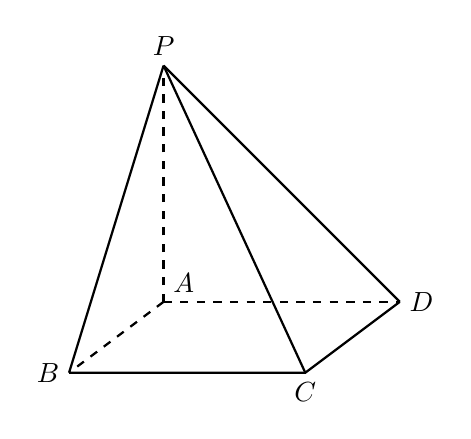
\begin{tikzpicture}[scale=1.5, >=latex]
		% 1. 定义顶点坐标（斜二测透视效果）
		\coordinate (A) at (0,0);
		\coordinate (B) at (-0.8,-0.6);
		\coordinate (C) at (1.2,-0.6);
		\coordinate (D) at (2,0);
		\coordinate (P) at (0,2);
		
		% 2. 绘制不可见线（虚线段）
		\draw[dashed, thick] (A) -- (B);
		\draw[dashed, thick] (A) -- (D);
		\draw[dashed, thick] (A) -- (P);
		
		% 3. 绘制可见线（实线段）
		\draw[thick] (B) -- (C) -- (D);
		\draw[thick] (P) -- (B);
		\draw[thick] (P) -- (C);
		\draw[thick] (P) -- (D);
		
		% 4. 标注顶点字母（带有微调方向，防止压线）
		\node[above] at (P) {$P$};
		\node[above right] at (A) {$A$};
		\node[left] at (B) {$B$};
		\node[below] at (C) {$C$};
		\node[right] at (D) {$D$};
	\end{tikzpicture}
	
	\kaodian{空间向量与立体几何-点线面之间的位置关系-空间点、直线、平面之间的位置关系-异面直线所成的角}
\end{example}

\begin{example}{4}[2025][新高考1卷][高三][高考][第18题]
	设椭圆$C:\dfrac{x^2}{a^2}+\dfrac{y^2}{b^2}=1(a>b>0)$的离心率为$\dfrac{2\sqrt{2}}{3}$，下顶点为$A$，右顶点为$B$，$|AB|=\sqrt{10}$.
	\begin{enumerate}
		\item 求椭圆的标准方程；
		\item 已知动点$P$不在$y$轴上，点$R$在射线$AP$上，且满足$|AR|\cdot|AP|=3$.
		\begin{enumerate}
			\item 设$P(m,n)$，求点$R$的坐标（用$m$，$n$表示）；
			\item 设$O$为坐标原点，$M$是椭圆上的动点，直线$OR$的斜率为直线$OP$的斜率的$3$倍，求$|PM|$的最大值.
		\end{enumerate}
	\end{enumerate}
	\kaodian{空间向量与立体几何-圆锥曲线-直线与圆锥曲线的位置关系-椭圆中的参数范围及最值}
\end{example}

\begin{example}{4}[2025][新高考1卷][高三][高考][第19题]
	\begin{enumerate}
		\item 设函数$f(x)=5\cos x-\cos5x$，求$f(x)$在$\left[0,\dfrac{\pi}{4}\right]$的最大值；
		\item 给定$\theta\in(0,\pi)$，设$a$为实数，证明：存在$y\in[a-\theta,a+\theta]$，使得$\cos y\le\cos\theta$；
		\item 若存在$\varphi$使得对任意$x$，都有$5\cos x-\cos(5x+\varphi)\le b$，求$b$的最小值.
	\end{enumerate}
	\kaodian{导数与函数-导数及其应用-导数在研究函数中的作用-利用导数求最值}
\end{example}
	\end{document}